\section{Structure of the LHCb Detector}
The Large Hadron Collider beauty (LHCb) detector is a single-arm spectrometer possessing a forward angular coverage from
approximately 10 mrad to 300 (250) mrad in the bending (non-bending) plane \cite{https://doi.org/10.48550/arxiv.0910.1740}
The structure of the detector is motivated by the fact that both the $b$ and the $\bar{b}$ hadrons are predominantly produced in the
same forward or backward cone. The components that enable the identification of particles, and aid the deduction of their properties include
the vertex locator system (VELO), the tracking system, comprising of a Trigger Tracker (a silicon microstrip detector, TT) located in front 
of the magnet, three tracking stations behind the magnet made up of silicon microstrips in the inner and outer parts (labelled IT and OT respectively),
two Ring Imaging Cherenkov counters (labelled RICH1 and RICH2 respectively), as well as a calorimeter system, comprising of a Scintillating Pad Detector and Preshower
(SPD/PS) and electromagnetic and hadronic calorimeters (ECAL and HCAL respectively) \cite{https://doi.org/10.48550/arxiv.0910.1740}. The layout of the LHCb spectrometer including the relative positions of the components described above, is illustrated in Figure \ref{LHCbDetector}.\\
\\
Of the abovementioned components, the dipole magnet, VELO, and ECAL play a significant role
in the analysis of the decay described in Section \ref{DecayProcess}. The structure of these sections of the
detector is further elaborated on in the sections that follow.
\begin{figure}[H]
    \centering
    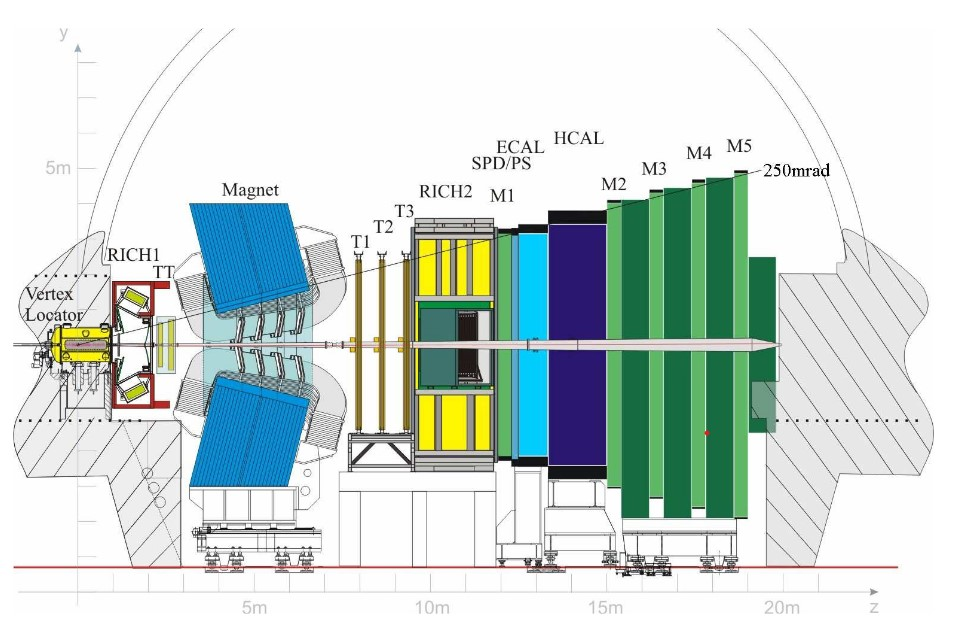
\includegraphics[scale = 0.45]{LHCbDetector.jpg}
    \caption{Diagram of the LHCb detector illustrating its various components. The coordinate system is oriented such that the beam is directed along the $z$ axis, and the $y$ axis is oriented along the vertical. Figure sourced from \cite{AbellanBeteta:2020amj}}
    \label{LHCbDetector}
\end{figure}
\subsection{Vertex Locator (VELO)}
The Vertex Locator (VELO) is a silicon-tracking detector in the spectrometer of the LHCb experiment shown in Figure (\ref{LHCbDetector}) above, and is responsible for the high-precision reconstruction of the primary and secondary vertices, and impact parameters of particle decays. In addition to this, it is a key
contributor to the measurements of particle lifetimes \cite{Kopciewicz_2022}.
\subsubsection{Angular Coverage}
\subsubsection{Triggering}
\subsubsection{Reconstruction Efficiency}
\subsubsection{Displaced Tracks and Vertices}
\subsubsection{Decay Time}
\subsection{Ring Imaging Cherenkov (RICH) Detector}
\subsection{Magnet} 
A warm dipole magnet is employed within the design of the LHCb in order to measure the momenta of charged particles. This measurement 
encompasses the forward acceptance of $\pm$ 250 mrad vertically and of $\pm$ 300 mrad horizontally
\subsection{Electromagnetic Calorimeter (ECAL)}
The ECAL thickness of 25 radiation lengths ensures the complete
containment of the high energy elecctromagnetic showers, as well as the acquisition
of an optimal energy resolution. The structure of the ECAL cells, comprising of 2 mm layers of lead and 4 mm scintillator layers is demonstrated in
Figure \ref{ECALStructure} below. The cells are said to have a "shashlik" structure, and the scintillation light readout is performed by Hamamatsu-R7899-20 photomultipliers \cite{AbellanBeteta:2020amj}. 
The ECAL comprises of a total of 6016 cells.
\begin{figure}[H]
    \centering
    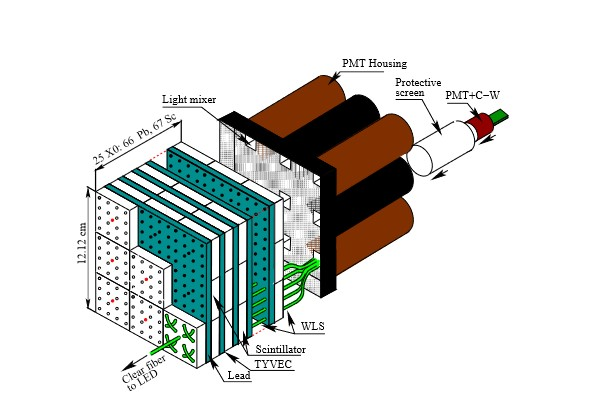
\includegraphics[scale = 0.75]{ECALStructure.jpg}
    \caption{ECAL cell. Figure sourced from \cite{AbellanBeteta:2020amj}}
    \label{ECALStructure}
\end{figure}
\section{Data Analysis at the LHCb}
The Large Hadron Collider provides proton-proton collisions to the LHCb approximately 40 million times per second, thereby generating a significant amount of data. In order to retain the data from events that are deemed to be of interest for analyses, the plethora of data must be filtered efficiently, and the algorithms
implemented must be sufficiently intricate, so as to be able to manage the complexity of the data being processed. The LHCb experiment implements a data flow which enables the aforementioned objectives to be addressed. The flow of data through the LHCb system is further detailed in the sections that follow.
\subsection{The LHCb Data Flow}\label{LHCbDataFlow}
The collision events recorded by the LHCb detector proceed through various steps, each of which is controlled by an application that processes the data in a way that maximises the efficiency of data acquisition and also enhances the quality of the obtained. The data from the detector is first filtered through hardware and software components, known as the L0 trigger, and the high level trigger (HLT) respectively. Following this, the data is
reconstructed to transform the detector into objects such as tracks and clusters, which are stored in an output file in a 'DST' format. Data from this files is further filtered through a set of selections known as the stripping, the output of which is produced in either a DST or a '$\mu$DST' (micro-DST) format.\\
\\
A substantial amount of Monte Carlo (MC) simulated data is also generated in parallel to the detector data as part of the data flow. This is processed in a very similar manner to the detector data outlined above. Figure \ref{LHCbData} illustrates the abovementioned stages of the data flow and processing. The framework implemented to generate and process the simulated events described above, along with its constituent components are further elaborated upon in the subsequent sections
\begin{figure}[H]
    \centering
    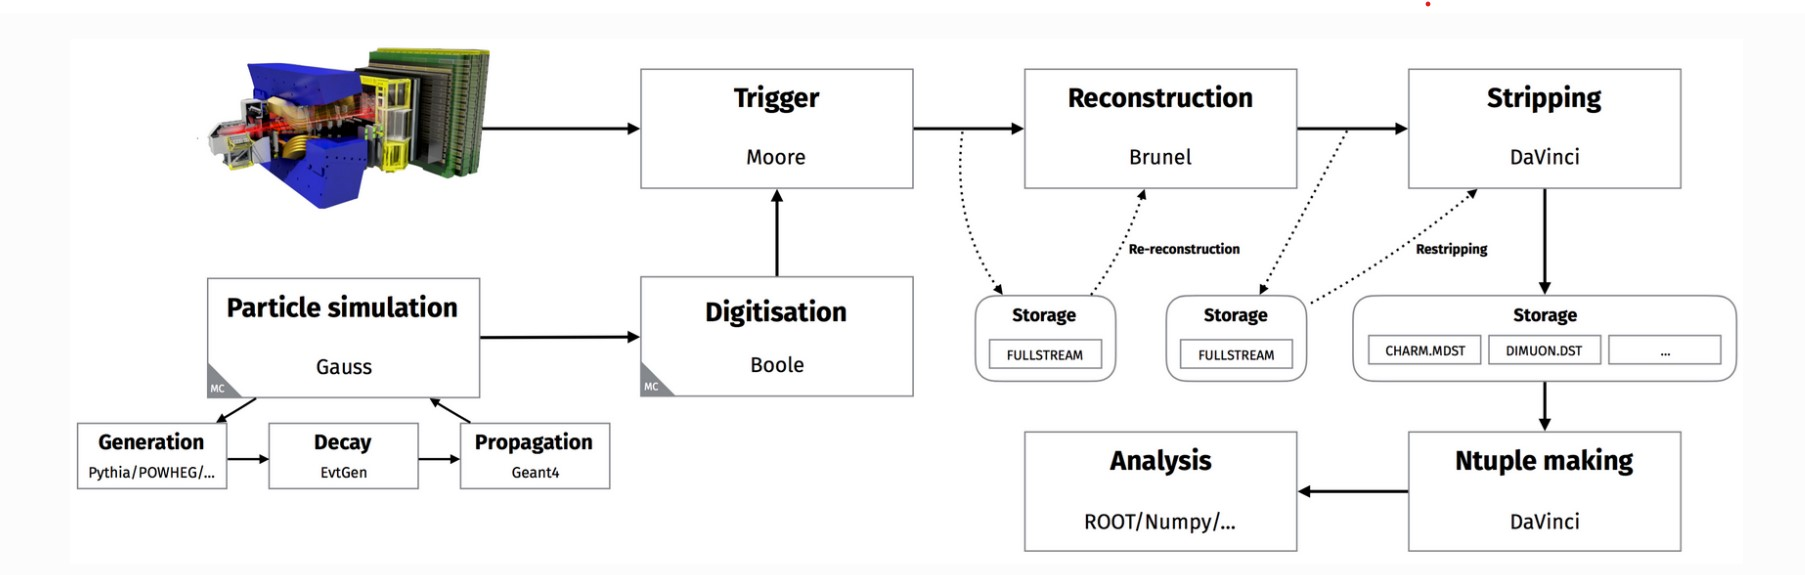
\includegraphics[scale = 0.4]{LHCbDataFlow.jpg}
    \caption{LHCb Data Flow}
    \label{LHCbData}
\end{figure}

\subsection{The LHCb Simulation Framework}
The MC simulated data that is processed in parallel to the detector data flows through a similar pipeline to its counterpart, with necessary steps in place to mimic the proton-proton collisions and the detector response. The former, and the subsequent hadronisation and decay of the resultant particles 
are controlled by the Gauss application, which is responsible for calling the various compatible Monte Carlo generators such as Pythia and POWHEG, as well as to control applications such as EvtGen and Geant4, which describe the decays of simulated particles and simulate their traversal through and interaction with
the detector. On the other hand, the latter entails the transformation of the simulated hits made in the virtual detector into signals that mimic the real detector. This process is regulated by the Boole application, whose output is designed to closely match that of the real detector, such that the simulated data produced can be 
processed via the process described in Section \ref{LHCbDataFlow} above. 
\subsubsection{Gauss}
\subsubsection{EvtGen}
\subsubsection{Pythia}
\subsubsection{Geant4}
\subsubsection{Boole} 



